\section{Vorwort}
Bei der Recherche zur Bearbeitung der Übungen wurden viele englischsprachige Webseiten zu rate gezogen. Generell kann man sagen, dass englische Fachbegriffe sich im Bereich FPGA und embedded Design etabliert haben, so dass eine Übersetzung eher verwirren als helfen würde. Daher haben wir uns entschieden, die \textbf{englischen} Bezeichner und Beschreibungen beizubehalten.\\
Um Codeabschnitte besser von Beschreibungen besser unterscheiden zu können, wurde eine eigene Schriftart verwendet:
\begin{verbatim}
  Kommandozeilen Eingaben und Codesnippets werden wie HIER dargestellt.
\end{verbatim}

\section{Aufgabe 1} \label{ex1}
In der Laborübung wurde das ZedBoard Zynq-7000 eingesetzt. Es umfasst als \textbf{PL} den Artix-7 FPGA mit 85K Logic Cells (Device Z-7020, Part: XC7Z020) und als \textbf{PS} den Dual-core ARM Cortex-A9 MPCore™ mit 866 MHz.

\subsection{Interrupt-Verarbeitung}
Ein Interrupt kann auf einem, der drei folgenden Ursachen entspringen:
\begin{itemize}
  \item Hardware: TODO
  \item Software: TODO
  \item Exception: TODO
\end{itemize}

Es gibt drei Ursachen für Interrupts auf dem Zynq-Board. 
Der GIC (Gerneric Interrupt Controller) auf dem Zynq Soc verarbeitet Interrupt aus folgenden Quellen:
\begin{itemize}
  \item Software-generierte Interrupts: TODO
  \item Shared periphere Interrupts: TODO
  \item Private periphere Interrupts: TODO
\end{itemize}


Ablauf bei eintreten eines Interrupts, führt der Prozessor folgende Schritte durch: 
\begin{enumerate}
  \item Ein Interrupt wurde aktiviert und muss verarbeitet werden
  \item Der Prozessor stoppt den aktuell laufenden Thread
  \item Der Prozessor speichert alle Threaddaten auf dem Stack, um diese später wieder herzustellen
  \item Der Prozessor führt die Interrupt Service Routine aus, die festlegt, wie der Interrupt zu verarbeiten ist.
  \item Der Prozessor holt die Daten des angehaltenen Threads vom Stack und setzt seine Verarbeitung fort.
\end{enumerate}

 \subsection{Interrupt-Setup}
 
 TODO Programmschritte
 
 \begin{minipage}{\textwidth}
    \begin{center}        
        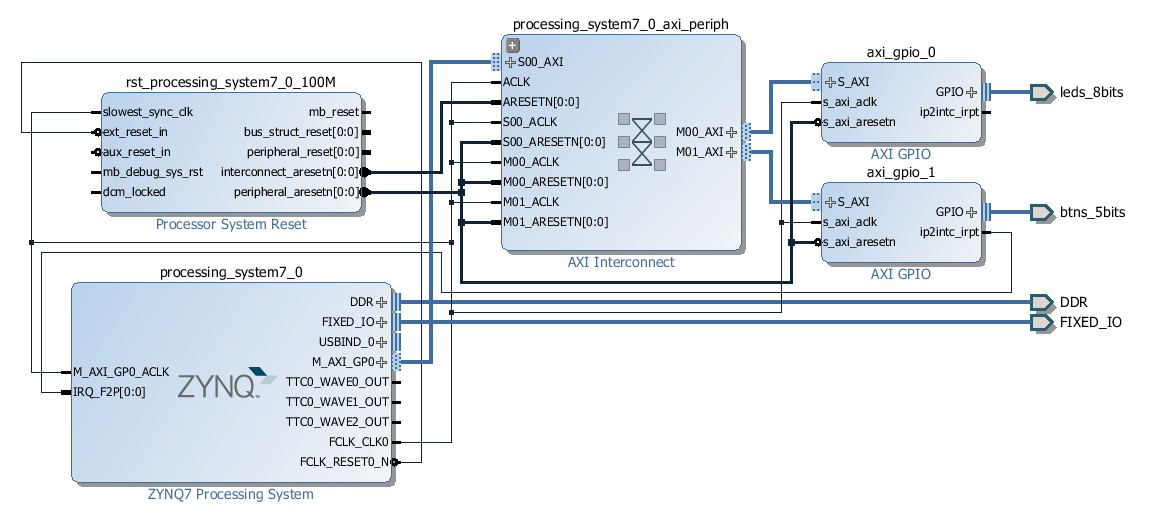
\includegraphics[scale=0.58]{img/lab2a1.png} 
    \end{center}
\end{minipage}
\begin{center}
Aufgabe Lab2 A1 Interrupt von GPio
\end{center}
 
 
 
\begin{verbatim}
   // IDs
   #define INTC_DEVICE_ID XPAR_PS7_SCUGIC_0_DEVICE_ID
   #define INTC_GPIO_INTERRUPT_ID XPAR_FABRIC_AXI_GPIO_1_IP2INTC_IRPT_INTR
 	
   XGpio IntrSource ; // e.g. source of interrupt gpio
   XScuGic INTCInst ;
   
  void FunktionPointerInterrServiceRout (void * InstancePtr) { /*interrupt  routine*/ }

  int main()  {
      XScuGic_Config * IntcConfig;
      // Interrupt controller initialisation
      IntcConfig = XScuGic_LookupConfig ( INTC_DEVICE_ID );
      // optional Status prUfen if XST_SUCCESS
      status = XScuGic_CfgInitialize (& INTCInst, IntcConfig,
                           IntcConfig -> CpuBaseAddress );
      // Call to interrupt setup       
     status = InterruptSystemSetup (& INTCInst );
     // Connect GPIO interrupt to handler
     status = XScuGic_Connect (& INTCInst , INTC_GPIO_INTERRUPT_ID ,
                ( Xil_ExceptionHandler ) FunktionPointerInterrServiceRout ,
                     ( void *) &IntrSource );
      // Enable GPIO interrupts interrupt
     XGpio_InterruptEnable ( &IntrSource , 1);
     XGpio_InterruptGlobalEnable ( &IntrSource );

     // Enable GPIO and timer interrupts in the controller
     XScuGic_Enable (& INTCInst , INTC_GPIO_INTERRUPT_ID );

     return 0;
   }
 \end{verbatim}